%!TEX root = chi14grammatical.tex

\begin{figure*}[th]
\begin{subfigure}{0.5\columnwidth}
		\begin{subfigure}{\columnwidth}
				\centering
		\fbox{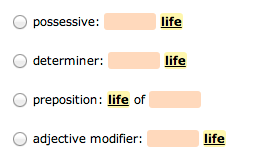
\includegraphics[width=\columnwidth]{fig/baseline-choices}}
	    \caption {The options as they appear in the \emph{baseline} condition. \label{fig:baseline-choices}}
	    \end{subfigure}

	    \begin{subfigure}{\columnwidth}
	    	\centering
	    	\fbox{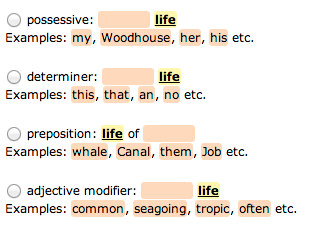
\includegraphics[width=\columnwidth]{fig/words-choices}}
	        \caption {The same options as they appear in the \emph{words} condition. \label{fig:words-choices}}
	    \end{subfigure}
\end{subfigure}
\quad
\begin{subfigure} {1.5\columnwidth}
			\centering
	\fbox{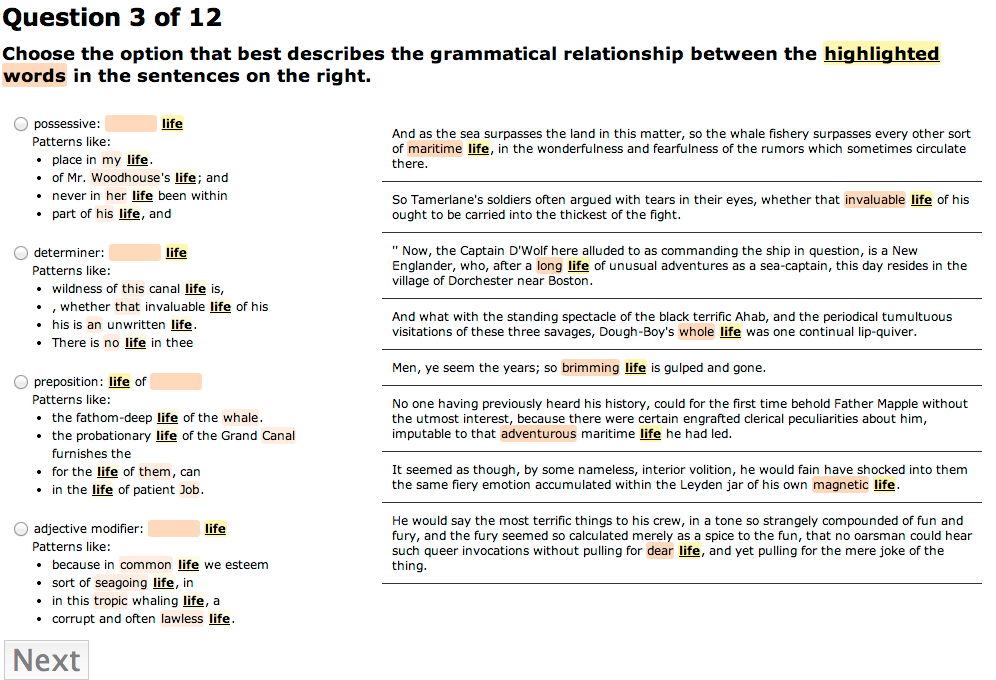
\includegraphics[width=\columnwidth]{fig/task}}
	\caption{\label{fig:task} The same options in the \emph{phrases} condition, shown as they appeared in an identification task for the relationship \code{amod(life, \_\_\_)} (where different adjectives modify the noun `life'). The correct answer is `adjective modifier' (4th option), and the remaining 3 options are distractors.}
	\end{subfigure}

\caption{\label{fig:choices} The appearance of the choices shown in the three experiment conditions.}
\end{figure*}


We gave participants a series of identification tasks. In each task, they were shown a list of sentences containing a particular syntactic relationship between highlighted words. They were asked to identify the relationship type from a list of four options. We presented the options in three different ways, and compared the accuracy.

We chose Amazon's Mechanical Turk (MTurk) crowdsourcing platform as a source of study participants. The wide range of backgrounds provided by MTurk is desirable because our goal is to find a representation that is understandable to most people, not just linguistic experts or programmers.  This platform has become widely used for both obtaining language judgements and for usability studies \cite{kittur2008crowdsourcing,snow2008cheap}.


Our hypothesis was:
\begin{quote}
	Grammatical relations are identified more accurately when shown with examples of contextualizing words or phrases than without.
\end{quote}

To test it, participants were given a series of identification tasks. In each task, they were shown a list of 8 sentences, each containing a particular relationship between highlighted words. They were asked to identify the relationship from a list of 4 choices.  Additionally, one word was chosen as a \emph{focus word} that was present in all the sentences, to make the relationship more recognizable (``life'' in Figure~\ref{fig:choices}).

The choices were displayed in 3 different ways (Figure \ref{fig:choices}).  The \strong{baseline} presentation
(Figure \ref{fig:baseline-choices}) named the linguistic relation and showed a blank space with a pink background for the varying word in the relationship, the focus word highlighted in yellow and underlined, and any necessary additional words necessary to convey the relationship (such as ``of" for the prepositional relationship ``of",  the third option).

The \strong{words} presentation showed the baseline design, and in addition beneath was the word ``Examples:'' followed by a list of 4 example words that could fill in the pink blank slot (Figure \ref{fig:words-choices}).   The \strong{phrases} presentation again showed the baseline design, beneath which was the phrase ``Patterns like:'' and a list of 4 example phrases in which fragments of text including both the pink and the yellow highlighted portions of the  relationship appeared (Figure \ref{fig:task}).

{\bf Method:} We used a between-subjects design. The task order and the choice order were not varied: the only variation between participants was the presentation of the choices. To avoid the possibility of  guessing the right answer by pattern-matching, we ensured that there was no overlap between the list of sentences shown, and the examples shown in the choices as words or phrases.

{\bf Tasks:} The tasks were generated using the Stanford Dependency Parser \cite{de2006generating} on the text of \emph{Moby Dick} by Herman Melville. We tested the 12 most common grammatical relationships in the novel in order to cover the most content and to be able to provide as many real examples as possible. These relationships fell into two categories, listed below with examples.

Clausal or long-distance relations:
\squishlist
	\item Adverbial clause: \emph{ I \textbf{walk} while \textbf{talking}}
	\item Open clausal complement:  \emph{I \textbf{love} to \textbf{sing} }
	\item  Clausal complement:  \emph{ he \textbf{saw} us \textbf{leave}}
	\item  Relative clause modifier:  \emph{the \textbf{letter} I \textbf{wrote} reached }
\squishend

Non-clausal relations:
\squishlist
	\item Subject of verb: \emph{\textbf{he} \textbf{threw} the ball}
	\item Object of verb:  \emph{ he \textbf{threw} the \textbf{ball}}
	\item Adjective modifier \emph{\textbf{red} \textbf{ball}}
	\item Preposition (in): \emph{a \textbf{hole} in a \textbf{bucket}}
	\item Preposition (of):  \emph{ the \textbf{piece} of \textbf{cheese}}
	\item Conjunction (and)  \emph{ \textbf{mind} and \textbf{body}}
	\item Adverb modifier: \emph{  we \textbf{walk} \textbf{slowly}}
	\item Noun compound:  \emph{ \textbf{Mr.}  \textbf{Brown}}
\squishend

We tested each of these 12 relations with 4 different focus words, 2 in each role. For example, the \emph{Subject of Verb} relation  was tested in the following forms:
\squishlist
	\item \code{(Ahab, \_\_\_)}:  the sentences each contained `Ahab', highlighted in yellow, as the subject of different verbs highlighted in pink.
	\item \code{(captain, \_\_\_)}

	\item \code{(\_\_\_, said)}: the sentences each contained the verb `said', highlighted in yellow, but with different subjects, highlighted in pink.
	\item \code{(\_\_\_, stood)}
\squishend

To maximize coverage, yet keep the total task time reasonable (average 6.8 minutes), we divided the relations above into 4 task sets, each testing recognition of 3 different relations. Each of relations was tested with 4 different words, making a total of 12 tasks per participant.

{\bf Participants:} 400 participants completed the study distributed randomly over the 4 task sets and the 3 presentations. Participants were paid 50c (U.S.) for completing the study, with an additional 50c bonus if they correctly identified 10 or more of the 12 relationships. They were informed of the possibility of the bonus before starting.

 To gauge their syntactic familiarity, we also asked them to rate how familiar they were with the terms `adjective' (88\% claimed they could define it), `infinitive' (43\%), and `clausal complement' (18\%). To help ensure the quality of effort, we included a multiple-choice screening question, ``What is the third word of this sentence?"  Those that answered incorrectly were eliminated.



\begin{figure}
\centering
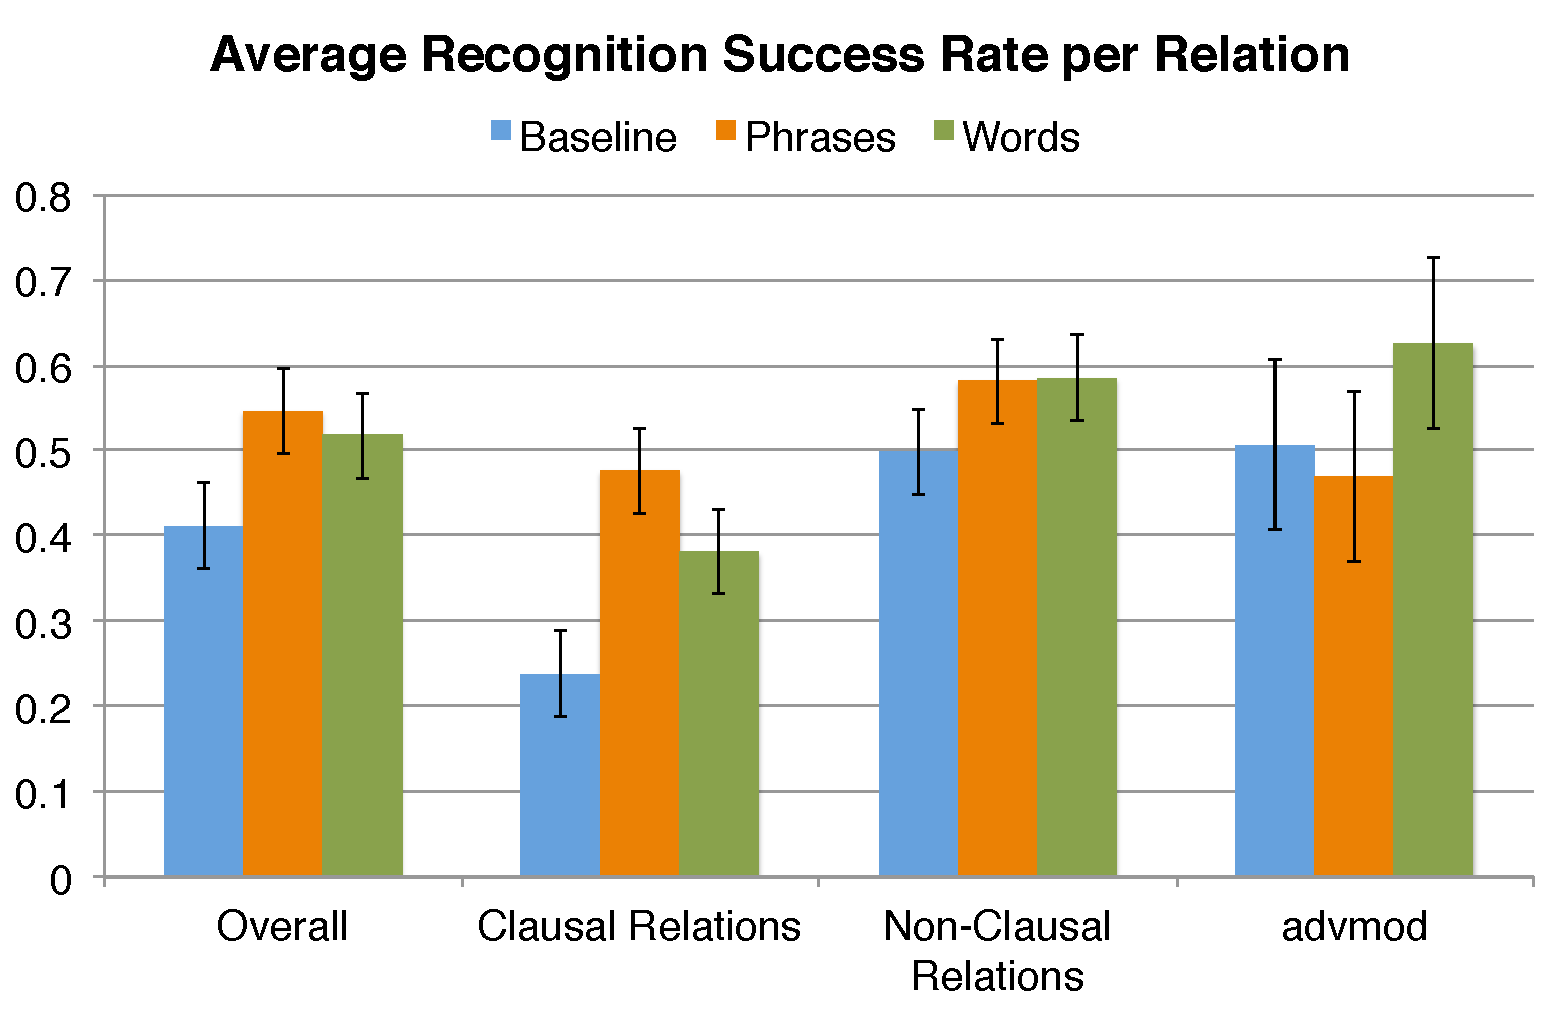
\includegraphics[width=\columnwidth]{fig/results}
\caption{\label{fig:results} Recognition rates for different types of relations under the 3 experiment conditions, with 95\% confidence intervals.}
\end{figure}

{\bf Results:} The results (Figure \ref{fig:results}) confirm our hypothesis. Participants in conditions that showed examples (\strong{phrases} and \strong{words}) were significantly more accurate at identifying the relations than participants in the \strong{baseline} condition. We used the Wilcoxson signed-rank test, an alternative to the standard T-test that does not assume samples are normally distributed. The average success rate in the \strong{baseline} condition was 41\%, which is significantly less accurate than \strong{words}: 52\%, (p=0.00019, W=6136), and \strong{phrases}: 55\%, (p=0.00014, W=5546.5).

Clausal relations operate over longer distances in sentences, and so it is to be expected that showing longer stretches of context would perform better in these cases; that is indeed what the results showed.
Phrases significantly outperformed words and baseline for clausal relations. The average success rate was 48\% for \strong{phrases}, which is significantly more than \strong{words}: 38\%, (p=0.017 W=6976.5) and \strong{baseline}: 24\%, (p=1.9$\times 10^{-9}$ W=4399.0), which was indistinguishable from random guessing (25\%). This is a  strong improvement, given that only 18\% of participants reported being able to define  `clausal complement'.

For the non-clausal relations, there was no significant difference between \strong{phrases} and \strong{words}, although they were both overall significantly better than the baseline (words: p=0.0063 W=6740, phrases: p=0.023 W=6418.5). Among these relations, adverb modifiers stood out (Figure \ref{fig:results}), because evidence suggested that \strong{words} (63\% success) made the relation more recognizable than \strong{phrases} (47\% success, p=0.056, W=574.0) -- but the difference was only almost significant, due to the smaller sample size (only 96 participants encountered this relation). This may be because the words are the most salient piece of information in an adverbial relation -- adverbs usually end in `ly' -- and in the phrases condition the additional information distracts from recognition of this pattern.
